\documentclass[a4paper,10pt]{scrartcl}
\usepackage[utf8]{inputenc}
\usepackage[T1]{fontenc}
\usepackage{booktabs}
\usepackage{import}
\usepackage{xspace}
\usepackage{enumitem}
\usepackage{cite}
\usepackage{graphicx}
\usepackage{tikz}
\usepackage{wrapfig}
\usepackage{pdflscape}
\usetikzlibrary{arrows}
\usetikzlibrary{fit}
\usetikzlibrary{calc}
\usepackage{float}
\usepackage{amssymb}
\usepackage{listings}
\usepackage[section]{placeins} % don't move figures beyond the next section heading

% this is needed for forms and links within the text
\usepackage{hyperref}

% Variables
\newcommand{\authorName}{
   Mohammed~Abu~Jayyab,
   Niklas~Baumstark,
   Tobias~Gräf,
   Amrei~Loose,
   Christoph~Michel
}
\newcommand{\authorNameEmph}{
  \textbf{ Mohammed~Abu~Jayyab},
   Niklas~Baumstark,
   Tobias~Gräf,
   Amrei~Loose,
   Christoph~Michel
}

\newcommand{\dateFirstVersion}{\today}
\newcommand{\customer}{Karlsruhe Institute of Technology}
\newcommand{\contractor}{A company}
\newcommand{\projectName}{Broadcast Encryption\xspace}

\newcommand{\doctitle}{\projectName (Validation document)}
\title{\doctitle}
\author{\authorName}
\date{\today}

% less margin
\usepackage[margin=2.5cm]{geometry}

% horizontal line
\newcommand{\HRule}{\rule{\linewidth}{0.5mm}}

% more beautiful lists
\setlist{noitemsep}
\renewcommand{\labelitemi}{$\bullet$}
\renewcommand{\labelitemii}{$\diamond$}

% create a shorter version for tables
\newcommand\addrow[2]{#1 &#2\\ }
\newcommand\addheading[2]{\textbf{\sffamily #1} &\textbf{\sffamily #2}\\ \hline}
\newcommand\tabularhead{\begin{tabular}{lp{13cm}}
\hline
}

\newcommand\addmulrow[2]{ \begin{minipage}[t][][t]{2.5cm}#1\end{minipage}%
   &\begin{minipage}[t][][t]{8cm}
    \begin{enumerate} #2   \end{enumerate}
    \end{minipage}\\ }

\newenvironment{usecase}{\tabularhead}
{\hline\end{tabular}}

% a cross
\newcommand\X{$\times$}

% templates and default styles for figures and graphics
\tikzset{>=triangle 45}
\tikzset{font=\sffamily}

\newcommand{\tmpCaption}{}
\newenvironment{illustration}[1]
{
   \renewcommand{\tmpCaption}{#1}
   \begin{figure}[h!]
   \centering
}
{
   \caption{\tmpCaption}
   \end{figure}
}


\begin{document}

\maketitle
  \begin{tabular}[t]{ll}
	Projekt:       & \quad \projektName \\[1.2ex]
	Auftraggeber:  & \quad \auftraggeber\\[1.2ex]
	Auftragnehmer: & \quad \auftragnehmer\\[1.2ex]
  \end{tabular}

\begin{tabular}{|p{3 cm}|p{3 cm}|p{5 cm}|}
\hline
\textbf{Version} & \textbf{Datum} & \textbf{Autor(en)} \\
\hline
\hline
1.0 & 29.04.2012 & \authorName \\
\hline
\end{tabular}

\tableofcontents
\clearpage

\section{Introduction}
This document describes procedures concerning the testing of our CryptoCast project for compliance with the requirements. The requirements that the software is to be verified against can be found in the functional specifications document. The goal of verifying and validating is to ensure that our system works correctly and meets its written specifications.

\section{Tests}
\subsection{Unit tests}
The goal we have towards unit testing is to cover all of the possible scenarios we can think of via test cases.

\subsubsection{cryptocast.crypto} This package provides basic primitives for working with broadcast encryption protocols and useful utilities for working with polynomials and elliptic curves over fields, which is necessary to implement the Naor-Pinkas scheme.
The implemented unit tests cover all the functionalities provided in the package, especially the polynomial and Langrange evaluation, modulo and elliptic curves computations and dynamic cipher streams generation.
\subsubsection{cryptocast.crypto.noarpinkas}
Contains tests for the Naor-Pinkas-based server and client implementations, including broadcasting and receiving encrypted streams using the Naor-Pinkas protocol.
\subsubsection{cryptocast.comm}
This package provides functionality related to communication between the different layers of the network protocol and to the communication between the server and clients. The unit tests in this package focus on the different stream-constructs regarding the send and receive functionality.
\subsubsection{cryptocast.util}
Has several unit tests for the general utility methods that are used throughout the project.
\subsubsection{cryptocast.server}
Tests in this package cover the server application implementation. Tests for managing the users and their keys as well as broadcasting are implemented here.

\subsubsection{cryptocast.server.programs}
The classes in this package were not tested, because they are not a part of the overall project. These programs just offer a convenient way of starting and benchmarking the server implementation.

\subsubsection{cryptocast.client}
Contains client tests that are implemented using the Robolectric framework, which allows running test suits using the Android API without an emulator. The client project doesn't have many logic tests, because it mainly uses the Android API without implementing any new logic. Besides, its components, cryptography and communication, are already tested in the before-mentioned packages \textit{cryptocast.crypto} and \textit{cryptocast.comm}.

\subsubsection{cryptocast.client.filechooser}
File chooser tests are implemented in this package and cover choosing a key file from the filesystem, that is handled by the FileChooserActivity.


\subsection{Test scenarios}
The test scenarios in the functional specifications document can be divided into two categories:

\begin{itemize}
	\item User Interface (UI) tests, which involve running the client on an Android device and testing specific functionalities regarding client-server interaction.
	\item Logic tests throughout the projects realized as unit tests based on JUnit. 
\end{itemize}

\subsection{User Interface Test Scenarios}

\subsubsection{/TF10/}
This scenario tests the normal program flow, where all actions are performed by an authorized user.

\begin{itemize}
	\item Actor: Client user.
	\item Start Constraints: User has a valid key, Server is streaming.
	\item Goal: User can receive and correctly view the stream.
	\item Program Flow:
	\begin{itemize}
   \item User starts the application.
   \item User enters the hostname and the portnumber.
   \item User chooses the key file.
   \item User plays the audio stream.
\end{itemize}
\end{itemize}
The test was successful.

\subsubsection{/TF15/}
This scenario tests the program flow, where all actions are performed by an revoked user.

\begin{itemize}
	\item Actor: Client user.
	\item Start Constraints: User has a invalid key, Server is streaming.
	\item Goal: User can not view the stream.
	\item Program Flow:
	\begin{itemize}
   \item User starts the application.
   \item User enters the hostname and the portnumber.
   \item User chooses the key file.
   \item An error message is displayed describing the problem and the user can not view the stream.
\end{itemize}
\end{itemize}
The test was successful.

\subsubsection{/TF60/}
This scenario tests a connection to an already visited server by an authorized user.

\begin{itemize}
	\item Actor: Client user.
	\item Start Constraints: User connected to a server before.
	\item Goal: User can receive and correctly view the stream without the need to choose the key file again.
	\item Program Flow:
	\begin{itemize}
   \item User starts the application.
   \item User enters the hostname and the portnumber.
   \item User plays the audio stream.
\end{itemize}
\end{itemize}
The test was successful.
\newpage

\subsubsection{/TF80/}
This scenario tests covers invalid input and actions taken by the user.

\begin{itemize}
	\item Actor: Client user.
	\item Start Constraints: User has a valid key, Server is streaming.
	\item Goal: User can receive and correctly view the stream.
	\item Program Flow:
	\begin{itemize}
   \item User starts the application.
   \item User enters a wrong hostname and the port number.
   \item An error message is displayed describing the problem.
 	 \item User corrects the hostname and the portnumber.
	 \item User chooses the key file.
   \item User plays the audio stream.
\end{itemize}
\end{itemize}
The test was successful.

\subsection{Logic Test Scenarios}

\subsubsection{/TF20/}
This scenario tests the key generation functionality in the server.

\begin{itemize}
	\item Actor: Server user.
	\item Start Constraints: none.
	\item Goal: New identities and private keys are assigned to all users.
	\item Program Flow:
	\begin{itemize}
   \item User starts the server.
   \item User initializes the server with a specific number of users that can be revoked.
\end{itemize}
\end{itemize}
The test was successful.

\subsubsection{/TF30/}
This scenario tests broadcast functionality in the server.

\begin{itemize}
	\item Actor: Server user.
	\item Start Constraints: Existing keys for the available users.
	\item Goal: Server streams the specified file as an encrypted stream.
	\item Program Flow:
	\begin{itemize}
   \item User starts the server.
   \item User chooses the mp3 file.
   \item Server starts streaming.
\end{itemize}
\end{itemize}
The test was successful.

\subsubsection{/TF40/}
This scenario tests revoke functionality in the server.

\begin{itemize}
	\item Actor: Server user.
	\item Start Constraints: Minimum one user with a key exist.
	\item Goal: The revoked user can no longer view the broadcasted stream.
	\item Program Flow:
	\begin{itemize}
   \item Start the server.
   \item Revoke a specific user.
   \item The revoked user can no longer encrypt the stream.
\end{itemize}
\end{itemize}
The test was successful.


\subsubsection{/TF50/}
This scenario tests add-user functionality in the server.

\begin{itemize}
	\item Actor: Server user.
	\item Start Constraints: none.
	\item Goal: New user is added and a new key is generated and assigned to this user.
	\item Program Flow:
	\begin{itemize}
   \item Start the server.
   \item Add a new user.
\end{itemize}
\end{itemize}
The test was successful.

\subsubsection{/TF70/}
This scenario covers illegal actions taken by the user.

\begin{itemize}
	\item Actor: Server user.
	\item Start Constraints: none.
	\item Goal: An error message is displayed describing the problem.
	\item Following illegal actions are covered:
	\begin{itemize}
   \item An existing user is added.
   \item A non-existing user is revoked.
   \item A non-existing user is unrevoked.
\end{itemize}
\end{itemize}
The test was successful.


\newpage
\section{Code Coverage}
This section describes the status of our code coverage evaluation tests. For code coverage measurement we used EclEmma.
EclEmma is an Eclipse plug-in that generates code coverage reports and provide simple trace information about test cases. Coverage is defined as a measure of the completeness of the set of test cases, based on the relation between the total sum of all instructions and methods to the total sum of all methods, that are called by the test cases.


\subsection{cryptocast.crypto}
The evaluation of the code coverage for the package cryptocast.crypto is as shown in the following figure.
It has 81.5\% of the methods covered.

\begin{illustration}{Code coverage for package cryptocast.crypto}
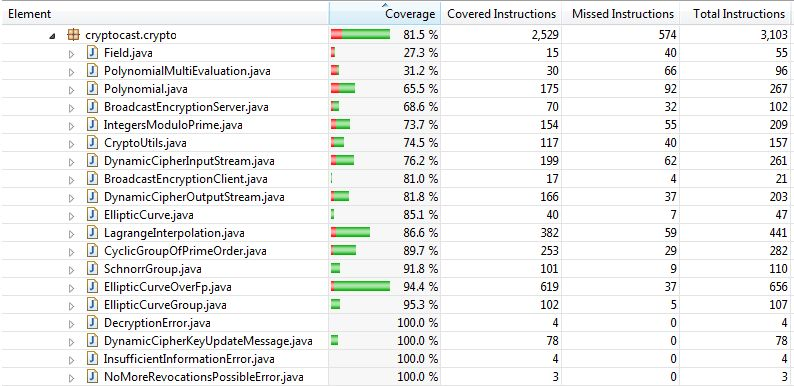
\includegraphics[width=450px]{figures/images/crypto.jpg}
\end{illustration}
\newpage

\subsection{cryptocast.crypto.noarpinkas}
The evaluation of the code coverage for the package cryptocast.crypto.noarpinkas is as shown in the following figure.
It has with 89.8\% of the methods covered.

\begin{illustration}{Code coverage for package cryptocast.crypto.noarpinkas}
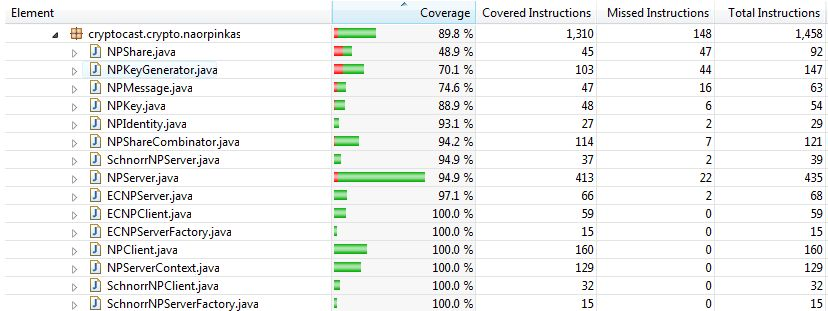
\includegraphics[width=450px]{figures/images/noarpinkas.jpg}
\end{illustration}

\subsection{cryptocast.comm}
The evaluation of the code coverage for the package cryptocast.comm is as shown in the following figure.
It has 63.9\% of the methods covered.

\begin{illustration}{Code coverage for package cryptocast.comm}
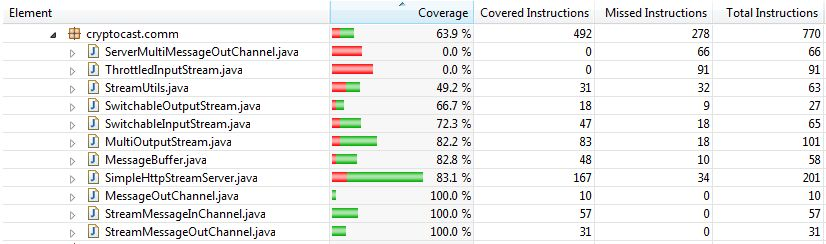
\includegraphics[width=450px]{figures/images/comm.jpg}
\end{illustration}
\newpage
\subsection{cryptocast.server}
The evaluation of the code coverage for the package cryptocast.server is as shown in the following figure.
It has 40.0\% of the methods covered. The server project is based entirely on the functionality provided by the crypto and communications parts, without implementing a lot of extra or new logic. The fact that can be reflected in the coverage results, whereby the 40\% of the covered code base corresponds to those parts where the additional logic was implemented. An automated tool can only provide an estimate based on static code analysis without taking the semantics of the code base into consideration, which is why these test coverage reports are considered a guideline.

\begin{illustration}{Code coverage for package cryptocast.server}
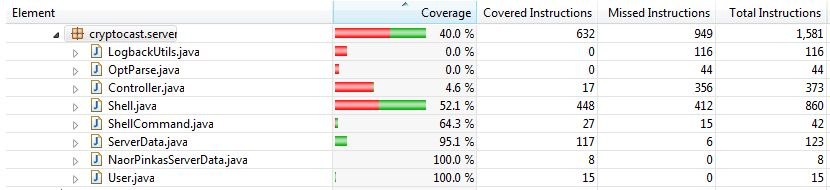
\includegraphics[width=450px]{figures/images/server.jpg}
\end{illustration}


\subsection{cryptocast.util}
The evaluation of the code coverage for the package cryptocast.util is as shown in the figure.
It has 39.8\% of the methods covered. The test coverage for the util project is relatively low, because most of the methods are convenience wrappers and helper functions around standard Java API.

\begin{illustration}{Code coverage for package cryptocast.util}
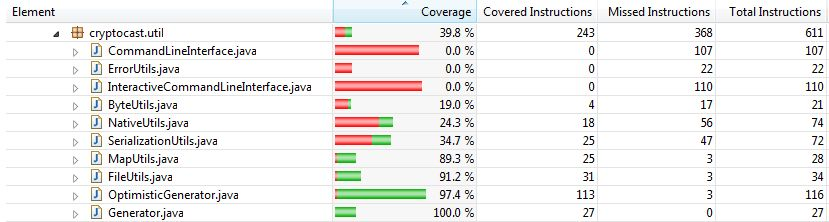
\includegraphics[width=450px]{figures/images/util.jpg}
\end{illustration}


\section{Conclusion}
Taking the User Interface tests into consideration in addition to the logic unit tests provides a wide spectrum of test coverage, that guarantees to a high degree a correct flow and robust implementation of the delivered applications.
  

\end{document}

